% bismi ALLAH ARAHMAN ARRAHIM




































\documentclass[11pt,a4paper]{article}

% ============================================================
% EX11 — Confirmatory validation of the Neural Core
% ============================================================

\usepackage[utf8]{inputenc}
\usepackage[T1]{fontenc}
\usepackage{lmodern}
\usepackage[a4paper,margin=2.15cm,headheight=14pt]{geometry}
\usepackage{microtype}
\usepackage{amsmath,amssymb,mathtools}
\usepackage{booktabs,tabularx,longtable,array}
\usepackage{enumitem}
\usepackage{graphicx}
\usepackage{float}
\usepackage{tikz}
\usepackage{ragged2e}
\usepackage{xcolor}
\usepackage{hyperref}
\usepackage{fancyhdr}
\usepackage{caption}
\usepackage{adjustbox}

\usetikzlibrary{
  arrows.meta,
  positioning,
  shapes.geometric,
  fit,
  backgrounds,
  calc
}

\hypersetup{
  colorlinks=true,
  linkcolor=blue!50!black,
  urlcolor=blue!50!black,
  citecolor=blue!50!black
}

\setlength{\parindent}{0pt}
\setlength{\parskip}{5pt}
\setlength{\emergencystretch}{3em}
\renewcommand{\arraystretch}{1.15}
\setlist[itemize]{leftmargin=1.5em,itemsep=2pt,topsep=3pt}
\setlist[enumerate]{leftmargin=1.7em,itemsep=2pt,topsep=3pt}

\pagestyle{fancy}
\fancyhf{}
\fancyhead[L]{EX11 -- Core neuronal}
\fancyhead[R]{Protocole confirmatoire}
\fancyfoot[C]{\thepage}

\newcommand{\CNG}{\textsc{CNG}}
\newcommand{\CNC}{\textsc{CNC}}
\newcommand{\RBF}{\textsc{AdaptiveRBF}}
\newcommand{\MAE}{\mathrm{MAE}}
\newcommand{\RMSE}{\mathrm{RMSE}}
\newcommand{\MSE}{\mathrm{MSE}}
\newcommand{\CoreN}{\textsc{Core neuronal}}
\newcommand{\Train}{\mathcal{D}_{\mathrm{train}}}
\newcommand{\Valid}{\mathcal{D}_{\mathrm{val}}}
\newcommand{\Test}{\mathcal{D}_{\mathrm{test}}}

\title{
  \textbf{EX11}\\
  Validation confirmatoire du core neuronal\\
  \large CNG multi-sondes et CNC par composition neuronale
}
\author{Projet th\_sondes}
\date{Version protocole -- à verrouiller avant exécution}

\begin{document}
\maketitle

\begin{abstract}
EX10 a montré qu'une composition de sondes neuronales adaptatives
peut apprendre certaines fonctions synthétiques et que des spécialistes
neuronaux peuvent être assemblés dans des graphes de calcul.
Les résultats restent toutefois limités par le nombre de familles de
fonctions, la profondeur des graphes, la généralisation à des structures
inédites et l'absence de preuve d'un avantage systématique sur les
modèles directs.

EX11 vise une validation confirmatoire du core neuronal.
Elle teste séparément : (i) la capacité multi-sondes du CNG,
(ii) la contribution fonctionnelle des sondes,
(iii) la composition CNC avec spécialistes gelés ou ajustés conjointement,
(iv) la généralisation à des fonctions et graphes non utilisés pour
l'entraînement, et (v) le coût logiciel d'exécution.

EX11 ne prétend pas valider le core logique adaptatif ni le core physique.
Ces deux couches restent hors du périmètre expérimental.
\end{abstract}

\tableofcontents
\newpage

% ============================================================
\section{Objectif scientifique et portée}
% ============================================================

\subsection{Question principale}

Le core neuronal est-il une architecture modulaire composée de sondes
adaptatives qui apporte une capacité de représentation, de composition
ou de réutilisation mesurable au-delà d'un modèle neuronal direct
de capacité comparable ?

L'expérience doit déterminer si les bénéfices observés dans EX10 :
\begin{itemize}
  \item se reproduisent sur plusieurs familles de fonctions ;
  \item persistent avec des graines et des échantillons indépendants ;
  \item résultent réellement de la présence de plusieurs sondes ;
  \item se transfèrent à des graphes de calcul non vus ;
  \item restent pertinents lorsque précision, paramètres et coût
        d'exécution sont comparés ensemble.
\end{itemize}

\subsection{Périmètre}

EX11 valide uniquement le \CoreN{} logiciel :
\begin{itemize}
  \item sondes neuronales adaptatives ;
  \item composition multi-sondes ;
  \item spécialistes neuronaux d'opérations ;
  \item apprentissage conjoint de graphes neuronaux ;
  \item généralisation fonctionnelle et compositionnelle.
\end{itemize}

EX11 ne valide pas :
\begin{itemize}
  \item la découverte automatique de graphes par un core logique ;
  \item la correction symbolique universelle des graphes ;
  \item une architecture matérielle dédiée ;
  \item un avantage énergétique ou industriel ;
  \item une supériorité générale sur les architectures neuronales existantes.
\end{itemize}

% ============================================================
\section{Hypothèses préenregistrées}
% ============================================================

\begin{longtable}{>{\RaggedRight\arraybackslash}p{0.12\textwidth}
                  >{\RaggedRight\arraybackslash}p{0.42\textwidth}
                  >{\RaggedRight\arraybackslash}p{0.36\textwidth}}
\toprule
\textbf{ID} & \textbf{Hypothèse} & \textbf{Critère de confirmation} \\
\midrule
H1 & Le CNG multi-sondes améliore la précision par rapport à une sonde
unique sur plusieurs familles de fonctions. &
Gain moyen apparié positif sur le test scellé, avec intervalle de
confiance excluant zéro sur le benchmark confirmatoire. \\
\addlinespace
H2 & Le CNG multi-sondes apporte un bénéfice au-delà d'une simple
augmentation de capacité. &
Au moins une configuration multi-sondes dépasse le MLP apparié en
paramètres sur plusieurs familles, sans dégradation majeure de
robustesse. \\
\addlinespace
H3 & Les sondes ont des contributions fonctionnelles mesurables. &
Les ablations produisent une dégradation reproductible, et les
contributions ne sont pas entièrement interchangeables entre sondes. \\
\addlinespace
H4 & Le CNC peut composer des spécialistes en graphes de calcul. &
Les graphes C2 obtiennent une erreur finie et reproductible, nettement
inférieure à C1 sur les graphes confirmatoires. \\
\addlinespace
H5 & La composition neuronale peut se généraliser à des graphes non vus. &
C2 transfère à des compositions retenues hors entraînement, avec une
erreur inférieure aux baselines composées non adaptées. \\
\addlinespace
H6 & Le core neuronal présente un compromis précision/coût utile. &
Au moins une configuration CNG ou CNC présente un compromis
non dominé en précision, paramètres et latence. \\
\bottomrule
\end{longtable}

Les hypothèses H1--H6 sont évaluées séparément. Un succès sur H1 ou H4
ne valide pas automatiquement H2, H3, H5 ou H6.

% ============================================================
\section{Modèle neuronal de base}
% ============================================================

\subsection{Sonde AdaptiveRBF}

Chaque sonde reçoit un vecteur d'entrée
$x\in\mathbb{R}^{p}$ et produit une sortie
$P(x)\in\mathbb{R}^{q}$.

Encodeur :
\[
z(x)=\tanh(W_e x+b_e), \qquad z\in\mathbb{R}^{d}.
\]

Centres RBF :
\[
c_k\in\mathbb{R}^{d},\qquad k=1,\ldots,K.
\]

Activations :
\[
r_k(x)=
\exp\left(
-\frac{\|z(x)-c_k\|_2^2}{2\sigma_k^2}
\right).
\]

Lecture :
\[
P(x)=V r(x)+b_r.
\]

Les centres sont initialisés par KMeans sur les seules représentations
du jeu d'entraînement. Les centres et largeurs sont entraînables.
Les largeurs sont paramétrées de manière à rester strictement positives
et bornées.

\subsection{Paramètres principaux}

Configuration principale :
\[
d=4,\qquad K=8.
\]

Analyse secondaire :
\[
d\in\{2,4,8\},\qquad K\in\{4,8,16\}.
\]

L'analyse secondaire est limitée à un sous-ensemble préenregistré de
tâches et ne peut pas remplacer les résultats principaux.

\subsection{Prétraitement}

Toute normalisation d'entrée est ajustée uniquement sur
$\Train$ et appliquée sans ré-estimation à $\Valid$ et $\Test$.

La normalisation des cibles, lorsqu'elle est utilisée dans une
expérience secondaire, est ajustée uniquement sur les cibles de
$\Train$. Les métriques finales sont toujours calculées dans les
unités originales.

Les opérations CNC utilisent des domaines mathématiques explicites.
Aucun échantillon invalide n'est silencieusement corrigé ou supprimé
après génération.

% ============================================================
\section{Plan expérimental général}
% ============================================================

\begin{figure}[H]
\centering
\begin{adjustbox}{max width=\textwidth}
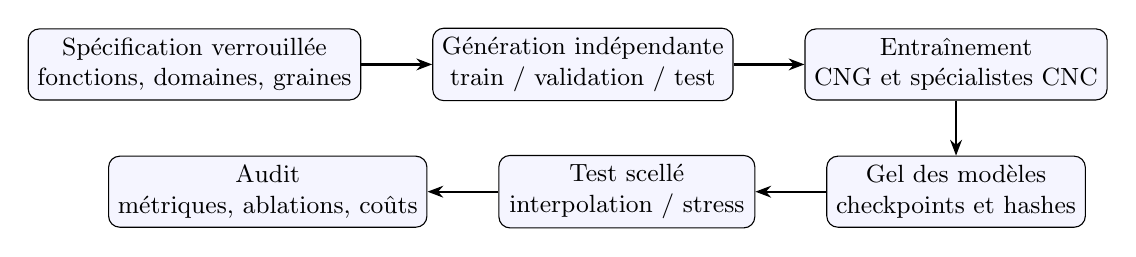
\begin{tikzpicture}[
  node distance=7mm and 9mm,
  box/.style={
    draw, rounded corners, align=center,
    minimum width=3.25cm, minimum height=0.85cm,
    font=\small, fill=blue!4
  },
  arr/.style={-{Stealth[length=2mm]},thick}
]
\node[box] (spec) {Spécification verrouillée\\fonctions, domaines, graines};
\node[box,right=of spec] (data) {Génération indépendante\\train / validation / test};
\node[box,right=of data] (fit) {Entraînement\\CNG et spécialistes CNC};
\node[box,below=of fit] (lock) {Gel des modèles\\checkpoints et hashes};
\node[box,left=of lock] (test) {Test scellé\\interpolation / stress};
\node[box,left=of test] (audit) {Audit\\métriques, ablations, coûts};

\draw[arr] (spec)--(data);
\draw[arr] (data)--(fit);
\draw[arr] (fit)--(lock);
\draw[arr] (lock)--(test);
\draw[arr] (test)--(audit);
\end{tikzpicture}
\end{adjustbox}
\caption{Pipeline confirmatoire EX11.}
\end{figure}

\subsection{Graines et répétitions}

Graines principales :
\[
\mathcal{S}=
\{1501,1607,1717,2029,3037,4099,4517,5003,6011,7013\}.
\]

Chaque graine détermine :
\begin{itemize}
  \item l'échantillonnage des données ;
  \item l'initialisation des paramètres ;
  \item l'initialisation KMeans ;
  \item l'ordre des mini-batches ;
  \item les opérations stochastiques éventuelles.
\end{itemize}

Les graines ne sont pas considérées comme des tâches indépendantes.
Les résultats sont rapportés par tâche et par graine, puis agrégés
avec des analyses appariées.

% ============================================================
\section{Partie A -- CNG multi-sondes}
% ============================================================

\subsection{Définition}

Pour une entrée $x$, le CNG exécute $M$ sondes :
\[
h_i=P_i(x),\qquad i=1,\ldots,M.
\]

Le vecteur concaténé est :
\[
h(x)=[h_1(x);\ldots;h_M(x)].
\]

Trois règles de composition sont évaluées :
\[
\hat f_{\mathrm{mean}}(x)=\frac{1}{M}\sum_{i=1}^{M}h_i(x),
\]
\[
\hat f_{\mathrm{learned}}(x)=W_c h(x)+b_c.
\]

Les sorties des sondes ont une dimension compatible avec la cible.
La moyenne fixe n'utilise aucun paramètre de composition.

\subsection{Configurations}

\begin{table}[H]
\centering
\small
\begin{tabularx}{\textwidth}{l c X}
\toprule
\textbf{ID} & \textbf{Sondes} & \textbf{Description} \\
\midrule
A1 & M=1 & AdaptiveRBF simple, référence neuronale. \\
A2 & M=2,4,7 & Moyenne fixe des sorties des sondes. \\
A3 & M=2,4,7 & Composeur linéaire appris sur les sorties concaténées. \\
A4 & -- & MLP direct apparié en nombre de paramètres. \\
A5 & -- & MLP direct de capacité supérieure, environ 4 fois les paramètres. \\
A6 & -- & AdaptiveRBF directe, sans multi-sondes. \\
\bottomrule
\end{tabularx}
\caption{Configurations CNG.}
\end{table}

\subsection{Familles de fonctions}

Les quatre tâches EX10 sont conservées comme benchmark de réplication :
\[
f_1(x)=\sin(x),\quad x\in[-\pi,\pi],
\]
\[
f_2(x_1,x_2)=x_1x_2,\quad (x_1,x_2)\in[-2,2]^2,
\]
\[
f_3(x_1,x_2)=x_1^2+x_2,\quad (x_1,x_2)\in[-2,2]^2,
\]
\[
f_4(x_1,x_2,x_3)=\sin(x_1x_2)+x_3,\quad
x\in[-2,2]^3.
\]

Deux familles confirmatoires supplémentaires sont introduites :
\[
f_5(x_1,x_2)=\sin(x_1)+0.5\cos(2x_2),
\]
\[
f_6(x_1,x_2,x_3)=x_1x_2+0.25x_3^2.
\]

Domaines :
\[
f_5:\ [-\pi,\pi]^2,\qquad
f_6:\ [-2,2]^3.
\]

Les fonctions $f_5$ et $f_6$ sont des tâches confirmatoires nouvelles.
Leurs résultats ne doivent pas être mélangés aux résultats de réplication
EX10 sans être également présentés séparément.

\subsection{Génération des données}

Pour chaque fonction et graine :
\begin{itemize}
  \item train : 4096 points tirés indépendamment du domaine primaire ;
  \item validation : 1024 points indépendants ;
  \item test scellé : 8192 points indépendants ;
  \item boundary test : points proches des frontières du domaine ;
  \item extrapolation : points dans un shell strictement extérieur.
\end{itemize}

Le shell d'extrapolation est défini par :
\[
\mathcal{X}_{\mathrm{extra}}
=
\left\{x:
x\in[-a-\delta,a+\delta]^p
\ \land\
x\notin[-a,a]^p
\right\},
\]
avec $\delta=1$ pour les domaines symétriques $[-a,a]^p$.

L'extrapolation est rapportée séparément et ne participe pas à la
sélection des modèles.

\subsection{Entraînement CNG}

Paramètres initiaux :
\begin{itemize}
  \item Adam, taux d'apprentissage $10^{-3}$ ;
  \item weight decay $10^{-5}$ ;
  \item batch size 128 ;
  \item maximum 800 epochs ;
  \item early stopping, patience 50 ;
  \item sélection du checkpoint par MAE validation ;
  \item même budget d'optimisation pour les configurations comparées.
\end{itemize}

Les hyperparamètres peuvent être modifiés uniquement avant le gel du
protocole. Toute modification postérieure est déclarée comme analyse
exploratoire.

% ============================================================
\section{Partie B -- Contribution et coopération des sondes}
% ============================================================

\subsection{Ablation leave-one-probe-out}

Pour chaque modèle A3 avec $M=4$ et $M=7$ :
\begin{enumerate}
  \item retirer une sonde $P_j$ ;
  \item geler les sondes restantes ;
  \item réapprendre uniquement le composeur ;
  \item comparer au modèle complet sur le même test scellé.
\end{enumerate}

La contribution de la sonde $j$ est :
\[
\Delta_j=
\MAE_{\mathrm{ablated}(j)}
-
\MAE_{\mathrm{full}}.
\]

Une valeur $\Delta_j>0$ indique que son retrait dégrade la précision.

\subsection{Deux régimes d'ablation obligatoires}

\textbf{Régime F -- sondes survivantes gelées :}
seul le composeur est réappris. Il mesure la contribution de la sonde
dans le système appris.

\textbf{Régime R -- système réduit réentraîné :}
les sondes restantes et le composeur sont réentraînés depuis une
initialisation indépendante. Il mesure si la capacité peut être
récupérée sans la sonde retirée.

Ces deux régimes ne doivent jamais être fusionnés dans une seule
statistique.

\subsection{Mesures de coopération}

Pour chaque tâche :
\begin{itemize}
  \item MAE/RMSE complète et ablatée ;
  \item $\Delta_j$ par sonde et par graine ;
  \item corrélation des erreurs entre sondes ;
  \item diversité des sorties des sondes ;
  \item stabilité des contributions entre graines ;
  \item nombre de sondes dont le retrait dégrade le modèle.
\end{itemize}

Une amélioration globale du modèle multi-sondes ne suffit pas à
démontrer une spécialisation. La spécialisation est considérée comme
soutenue seulement si les contributions et les profils d'erreurs
présentent une structure reproductible.

% ============================================================
\section{Partie C -- CNC par composition neuronale}
% ============================================================

\subsection{Principe}

Le CNC représente un graphe dirigé acyclique :
\[
G=(V,E).
\]

Chaque nœud $v\in V$ reçoit les sorties de ses prédécesseurs et produit
une approximation neuronale de son opération :
\[
\hat z_v=P_v(z_{u_1},\ldots,z_{u_k}).
\]

La cible finale est obtenue en propageant les sorties de nœuds jusqu'à
la sortie du graphe.

\subsection{Opérations spécialisées}

Les spécialistes de base sont :
\[
\{\mathrm{ADD,SUB,MUL,DIV,EXP,LOG}\}.
\]

Domaines de génération :
\begin{itemize}
  \item ADD, SUB, MUL : entrées primaires dans $[-2,2]$ ;
  \item DIV : numérateur dans $[-4,4]$, dénominateur dans
        $[-1,-0.25]\cup[0.25,3]$ ;
  \item EXP : entrée dans $[-2,2]$ ;
  \item LOG : entrée dans $[0.1,9]$.
\end{itemize}

Les données de chaque nœud sont générées depuis les entrées primaires
du graphe, puis propagées par les opérations exactes pour obtenir les
distributions des valeurs intermédiaires.

Les spécialistes ne sont pas entraînés sur des distributions
arbitraires indépendantes de leur contexte d'utilisation.

\subsection{Graphes de réplication EX10}

\[
g_1(a,b,c)=ab+\exp(c),
\]
\[
g_2(a,b,c)=\frac{ab}{c+1},
\]
\[
g_3(a,b,c)=\log(a^2+b^2+1)+\exp(c).
\]

Pour $g_2$, le domaine impose :
\[
|c+1|\geq 0.25.
\]

Pour $g_3$, l'argument du logarithme est toujours strictement positif.

\subsection{Graphes confirmatoires à composition inédite}

Deux graphes sont retenus hors entraînement :
\[
g_4(a,b,c)=\exp(ab)+c,
\]
\[
g_5(a,b,c)=\log(ab+5)+c^2,
\]
avec des domaines primaires garantissant les préconditions de
$\exp$, $\log$ et des divisions éventuelles.

Les graphes $g_4$ et $g_5$ ne sont pas utilisés pour sélectionner
les spécialistes, les hyperparamètres ou les checkpoints.
Ils testent la généralisation à une nouvelle composition d'opérations
connues.

\subsection{Configurations CNC}

\begin{table}[H]
\centering
\small
\begin{tabularx}{\textwidth}{l X}
\toprule
\textbf{ID} & \textbf{Description} \\
\midrule
C1 -- Frozen & Spécialistes préentraînés, gelés, assemblés sans
ajustement du graphe. \\
C2 -- Joint & Spécialistes initialisés depuis les checkpoints puis
ajustés conjointement sur les données du graphe. \\
C3 -- Direct MLP & MLP direct entraîné sur les entrées primaires
et la cible finale. \\
C4 -- Direct RBF & AdaptiveRBF directe entraînée sur les entrées
primaires et la cible finale. \\
C5 -- Native exact & Calcul exact des opérations, référence
mathématique non apprise. \\
\bottomrule
\end{tabularx}
\caption{Comparateurs CNC.}
\end{table}

\subsection{Séparation des données CNC}

Pour chaque graphe et graine :
\begin{itemize}
  \item train : 8192 entrées primaires ;
  \item validation : 2048 entrées primaires ;
  \item test scellé : 8192 entrées primaires ;
  \item boundary : entrées proches des limites admissibles ;
  \item stress : points admissibles proches des singularités ou
        régions de forte courbure.
\end{itemize}

Les données de test sont générées directement depuis les entrées
primaires. Les valeurs intermédiaires du test ne sont jamais utilisées
pour entraîner ou sélectionner un modèle.

\subsection{Propagation et erreur par nœud}

Pour chaque nœud $v$, calculer :
\[
e_v=\hat z_v-z_v^{\mathrm{exact}}.
\]

Au niveau final :
\[
e_{\mathrm{out}}=\hat y-y.
\]

Le rapport contient :
\begin{itemize}
  \item MAE/RMSE de chaque nœud ;
  \item MAE/RMSE de la sortie finale ;
  \item amplification ou atténuation de l'erreur ;
  \item contribution des erreurs de nœuds à l'erreur finale ;
  \item comparaison C1, C2, C3 et C4 sur les mêmes entrées primaires.
\end{itemize}

L'erreur relative n'est rapportée que lorsque la cible est éloignée
de zéro selon un seuil préenregistré. Elle ne remplace jamais MAE/RMSE.

% ============================================================
\section{Généralisation et tests scellés}
% ============================================================

\subsection{Niveaux de généralisation}

\begin{figure}[H]
\centering
\begin{adjustbox}{max width=\textwidth}
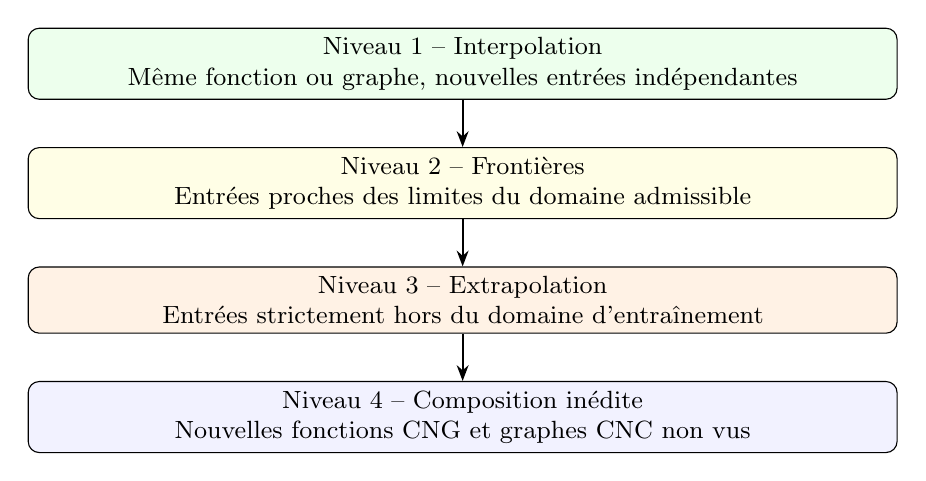
\begin{tikzpicture}[
  node distance=6mm,
  box/.style={
    draw,rounded corners,align=center,
    text width=10.8cm,minimum height=0.8cm,
    font=\small
  },
  arr/.style={-{Stealth[length=2mm]},thick}
]
\node[box,fill=green!7] (i) {Niveau 1 -- Interpolation\\
Même fonction ou graphe, nouvelles entrées indépendantes};
\node[box,below=of i,fill=yellow!10] (b) {Niveau 2 -- Frontières\\
Entrées proches des limites du domaine admissible};
\node[box,below=of b,fill=orange!10] (e) {Niveau 3 -- Extrapolation\\
Entrées strictement hors du domaine d'entraînement};
\node[box,below=of e,fill=blue!5] (c) {Niveau 4 -- Composition inédite\\
Nouvelles fonctions CNG et graphes CNC non vus};
\draw[arr] (i)--(b);
\draw[arr] (b)--(e);
\draw[arr] (e)--(c);
\end{tikzpicture}
\end{adjustbox}
\caption{Les quatre niveaux sont rapportés séparément.}
\end{figure}

\subsection{Règles de scellement}

Avant l'ouverture du test :
\begin{enumerate}
  \item figer le code et les configurations ;
  \item enregistrer les hashes des sources et checkpoints ;
  \item figer les listes de fonctions, graphes, graines et métriques ;
  \item enregistrer les prédictions du modèle sur validation ;
  \item verrouiller les modèles sélectionnés ;
  \item ouvrir le test scellé une seule fois pour l'analyse confirmatoire.
\end{enumerate}

Toute modification après ouverture du test est déclarée exploratoire
et nécessite un nouveau holdout indépendant pour une confirmation.

% ============================================================
\section{Métriques et analyse statistique}
% ============================================================

\subsection{Précision}

Pour $N$ exemples :
\[
\MAE=\frac{1}{N}\sum_{i=1}^{N}|\hat y_i-y_i|,
\]
\[
\RMSE=
\sqrt{\frac{1}{N}\sum_{i=1}^{N}(\hat y_i-y_i)^2}.
\]

Les résultats comprennent :
\begin{itemize}
  \item MAE et RMSE ;
  \item médiane et 90e percentile de l'erreur absolue ;
  \item erreurs par fonction, graphe et graine ;
  \item moyenne et écart-type entre graines ;
  \item différences appariées face aux baselines ;
  \item intervalles de confiance sur les différences.
\end{itemize}

\subsection{Comparaison appariée}

Pour une configuration candidate $A$ et une baseline $B$ :
\[
\Delta_s=\MAE_{B,s}-\MAE_{A,s}.
\]

Une valeur positive favorise $A$.

Les différences sont rapportées :
\begin{itemize}
  \item par tâche ;
  \item par graine ;
  \item en moyenne macro sur les tâches ;
  \item avec intervalle de confiance bootstrap apparié.
\end{itemize}

Les points de test ne sont pas traités comme des répétitions
indépendantes de l'entraînement. L'unité de répétition principale
est la graine, avec les tâches rapportées séparément.

\subsection{Critères d'interprétation}

\begin{itemize}
  \item \textbf{Soutien fort :} effet positif reproductible sur plusieurs
        tâches confirmatoires et intervalle de confiance de la
        différence excluant zéro.
  \item \textbf{Soutien limité :} gain sur certaines tâches seulement,
        ou effet incertain entre graines.
  \item \textbf{Non soutenu :} absence de gain reproductible ou
        performance inférieure aux comparateurs.
  \item \textbf{Non testé :} aucune expérience dédiée ne permet
        d'évaluer la proposition.
\end{itemize}

Aucun seuil de succès n'est modifié après consultation des résultats.

% ============================================================
\section{Coût et efficacité logicielle}
% ============================================================

Les coûts sont mesurés sur le même matériel, le même environnement
logiciel et le même nombre de threads.

Mesures :
\begin{itemize}
  \item nombre de paramètres entraînables ;
  \item taille des checkpoints ;
  \item mémoire maximale utilisée ;
  \item latence p50, p95 et p99 ;
  \item débit en exemples par seconde ;
  \item temps d'entraînement, rapporté séparément ;
  \item coût end-to-end incluant toutes les sondes et les nœuds.
\end{itemize}

Le temps d'entraînement n'est comparé que lorsque les conditions
d'exécution sont homogènes. Les mesures perturbées par concurrence
CPU sont marquées et exclues des comparaisons de vitesse.

Aucun avantage énergétique n'est revendiqué sans mesure directe
de consommation.

% ============================================================
\section{Critères d'arrêt et règles anti-biais}
% ============================================================

\begin{enumerate}
  \item Aucun choix de modèle à partir du test scellé.
  \item Aucun changement de domaine après observation des erreurs.
  \item Aucun remplacement silencieux des graines échouées.
  \item Toute divergence, NaN ou échec d'entraînement est conservé
        dans le journal d'exécution.
  \item Les comparateurs utilisent les mêmes partitions de données.
  \item Les budgets d'entraînement sont documentés et comparables.
  \item Les résultats négatifs sont inclus dans le rapport.
  \item Les résultats exploratoires sont séparés des résultats
        confirmatoires.
\end{enumerate}

Un run ne peut être déclaré complet que si son fichier de configuration,
son checkpoint, ses prédictions, ses métriques et son statut d'exécution
sont présents et cohérents.

% ============================================================
\section{Structure de livraison}
% ============================================================

\begin{verbatim}
EX11/
  README_EX11.md
  theory/
    EX11_NEURAL_CORE_PROTOCOL.tex
  configs/
    cng/
    cnc/
  src/
    models/
    data/
    train_cng.py
    train_cnc.py
    evaluate.py
    audit.py
  tests/
    test_domains.py
    test_data_leakage.py
    test_graph_execution.py
    test_metrics.py
  results/
    raw/
    checkpoints/
    predictions/
    metrics/
    processed/
  reports/
    CNG_CONFIRMATORY_REPORT.md
    CNC_CONFIRMATORY_REPORT.md
    EX11_FINAL_REPORT.md
  checksums/
    EX11_MANIFEST.json
    EX11_SHA256SUMS.txt
\end{verbatim}

% ============================================================
\section{Interprétation vis-à-vis de la vision globale}
% ============================================================

EX11 peut soutenir la composante neuronale de la vision si elle montre
que les sondes :
\begin{itemize}
  \item forment des modèles multi-sondes compétitifs ;
  \item apportent des contributions mesurables ;
  \item se composent dans des graphes de calcul ;
  \item transfèrent à des compositions non vues ;
  \item présentent un compromis précision/coût pertinent.
\end{itemize}

Même en cas de succès, les conclusions restent limitées au core neuronal.

\textbf{Core logique :} EX11 utilise des graphes fournis et ne teste pas
leur découverte, leur réécriture ou leur vérification automatique.

\textbf{Core physique :} EX11 mesure une exécution logicielle et ne
démontre pas d'avantage matériel, énergétique ou distribué.

\textbf{Intégration des trois cores :} elle nécessite une campagne
ultérieure où un core logique choisit ou vérifie le graphe, un core
neuronal fournit les modules de calcul, et un core physique exécute
ce graphe sous contraintes de ressources.

% ============================================================
\section{Conclusion attendue}
% ============================================================

EX11 est conçue pour répondre à une question précise :

\begin{quote}
Le core neuronal est-il une architecture modulaire et composable qui
apporte un bénéfice mesurable au-delà d'une collection de modèles
neuronaux indépendants ?
\end{quote}

Une réponse positive exige plus qu'une MAE faible sur quelques fonctions.
Elle exige des gains reproductibles, une contribution réelle des sondes,
une composition CNC robuste, une généralisation à des graphes non vus
et une comparaison honnête des coûts.

Si ces critères sont satisfaits, EX11 fournira une preuve expérimentale
plus forte de la faisabilité du core neuronal. Elle constituera alors
une base justifiée pour étudier l'intégration avec le core logique et
le core physique, sans prétendre les avoir déjà validés.

\end{document}